%!TEX program = xelatex
\documentclass[xcolor={table}]{beamer}

\usepackage[brazil]{babel}	
\usepackage[utf8]{inputenc}
\usepackage[T1]{fontenc}
\usepackage[scaled]{helvet}
\usepackage{amsthm}
\usepackage{ragged2e}
\usepackage{subfig}
\usepackage[table]{xcolor}
\usepackage{multicol}
\usepackage{multirow}
\usepackage{fancyvrb}
\usepackage{verbatim}
\usepackage{booktabs}
\usepackage{hyperref}
\usetheme{Execushares}
\usepackage{xcolor}
% \usepackage{floatrow}

\title{Emotion Detection in Speech}
% \subtitle{Flatiron School, Data Science, Flex Program}
\author{Milad Shirani}
\date{August 2022}

\setcounter{showSlideNumbers}{1}

\begin{document}
	\setcounter{showProgressBar}{0}
	\setcounter{showSlideNumbers}{0}
	
%%%%%%%%%%%%%%%%%%%%%%%%%%
%%%%%%%%%%%%%%%%%%%%%%%%%%
%%%%%%%%%%%%%%%%%%%%%%%%%%
%%%%%%%%%%%%%%%%%%%%%%%%%%
%%%%%%%%%%%%%%%%%%%%%%%%%%
%%%%%%%%%%%%%%%%%%%%%%%%%%

	\frame{\titlepage}

	\begin{frame}
		\frametitle{Contents}
		\begin{itemize}
			\item Project Overview 
			\item Data 
			\item Modeling and Results
% 			\item Interpretation of Coefficients
% 			\item Suggestions
			\item Q \& A
		\end{itemize}
	\end{frame}

	\setcounter{framenumber}{0}
	\setcounter{showProgressBar}{1}
	\setcounter{showSlideNumbers}{1}
	
%%%%%%%%%%%%%%%%%%%%%%%%%%%		
%%%%%%%%%%%%%%%%%%%%%%%%%%%	

		\begin{frame}
			\frametitle{Project Overview}
			\begin{enumerate}
			    \item In order for a therapist to fully analyze a patience, both words and emotions conveyed by patient's speech is important.
			 %   \item In order for a therapist to fully analyze a patience, not only are the sentences important, but also the emotion conveyed by speech is important.
			    \item In this work, we want to introduce a new model to detect the emotion of an audio file.
				\item We used Convolutional Neural Network as well as Transfer Learnings such as \textcolor{blue}{\href{https://www.tensorflow.org/api_docs/python/tf/keras/applications/efficientnet/EfficientNetB3}{EfficientNetB3}} and \textcolor{blue}{\href{https://www.tensorflow.org/api_docs/python/tf/keras/applications/efficientnet/EfficientNetB7}{EfficientNetB7}}
			\end{enumerate}
		\end{frame}
%%%%%%%%%%%%%%%%%%%%%%%%%%%		
%%%%%%%%%%%%%%%%%%%%%%%%%%%
\begin{frame}{Data and Method}
\begin{itemize}
    \item 2800 audio files provided by 
     \textcolor{blue}{\href{https://tspace.library.utoronto.ca/handle/1807/24487}{University of Toronto}} 
     
     \begin{figure}
        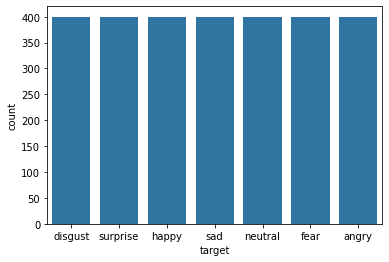
\includegraphics[width=0.5\linewidth]{distribution.png}
        \captionof{}{Distribution of Categories}
    \end{figure}
     
    \item Converting audio files to mel-spectrograms
    \end{itemize}
   
\end{frame}

%%%%%%%%%%%%%%%%%%%%%%%%%%%		
%%%%%%%%%%%%%%%%%%%%%%%%%%%
\begin{frame}\frametitle{Effects of Denoising}

\vspace{0.7cm}
\begin{figure}
  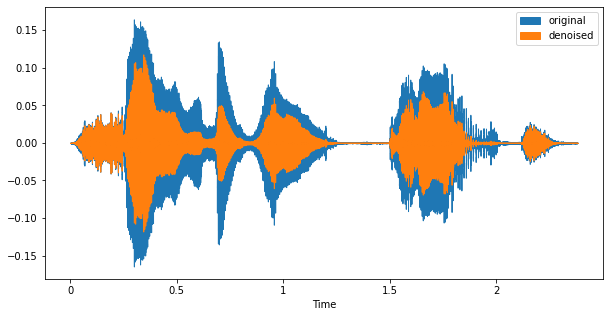
\includegraphics[width=0.5\linewidth]{original-denoised.png}
  \captionof{}{The Original and Denoised values of an Audio File}\par
  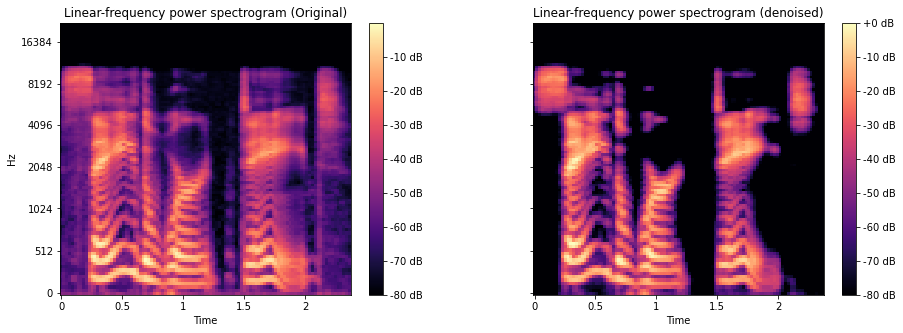
\includegraphics[width=0.8\linewidth]{spectrogram.png}
  \captionof{}{Mel-Spectrograms of Original and Denoised of an Audio File}
\end{figure}

\end{frame}



%%%%%%%%%%%%%%%%%%%%%%%%%%%
%%%%%%%%%%%%%%%%%%%%%%%%%%%


%%%%%%%%%%%%%%%%%%%%%%%%%%%		
%%%%%%%%%%%%%%%%%%%%%%%%%%%
\begin{frame}\frametitle{Effects of emotion}

\vspace{0.7cm}
\begin{figure}
  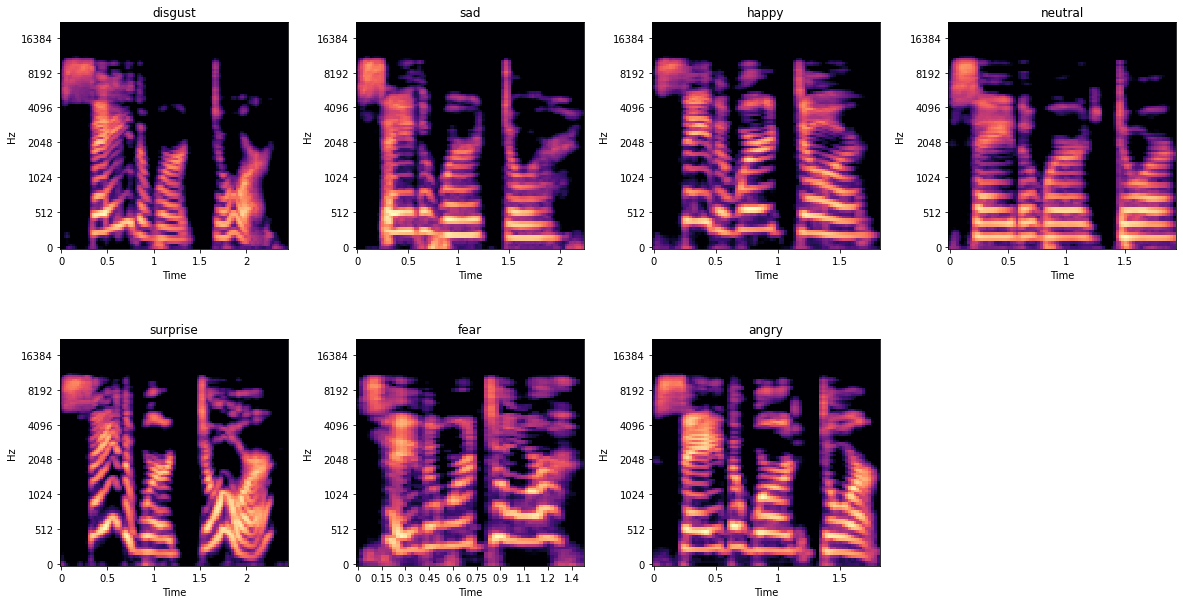
\includegraphics[width=1.05\linewidth]{door.png}
  \captionof{}{Effects of emotion in saying the word "door"}
  
\end{figure}

\end{frame}



%%%%%%%%%%%%%%%%%%%%%%%%%%%
%%%%%%%%%%%%%%%%%%%%%%%%%%%

% \begin{frame}{Modeling And Results}

% \begin{columns}[t]
%         \column{.5\textwidth}
%         \includegraphics[width=\columnwidth]{news_with_urls.png}
%         \captionof{}{Original and Denoised Audio Files}
%         \column{.5\textwidth}
%         \includegraphics[width=\columnwidth]{totanl_num_of_urls_in_each_news_category.png}
%         \captionof{}{Mel-Spectrograms}
%     \end{columns}

    
% \end{frame}


%%%%%%%%%%%%%%%%%%%%%%%%%%%		
%%%%%%%%%%%%%%%%%%%%%%%%%%%
\begin{frame}
\frametitle{Modeling and Results}
\vspace{0.5cm}
\begin{enumerate}
    \item Most of the deep learning models performed well with test accuracy of 99\% 
    % (expect EfficientNetB7 which has the lowest test accuracy which is about 0.95\% after 35 epochs).
    \item We would recommend the first CNN model (\textcolor{blue}{\href{https://github.com/miladshiraniUCB/Emotion-Detection-in-Speech/blob/main/Notebook/Modeling-CNN-and-Transfer-Learning.ipynb}{link to the model}}) because it has the simplest structure
    % and converges after 2 epochs as shown below
\end{enumerate}    


\begin{figure}%{0.4\linewidth}
  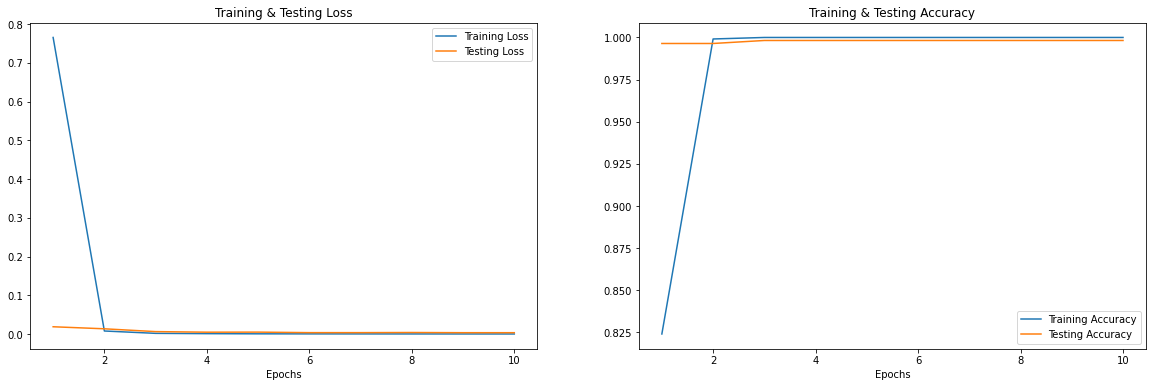
\includegraphics[width=0.9\linewidth]{results.png}
\end{figure}

\end{frame}

%%%%%%%%%%%%%%%%%%%%%%%%%%%		
%%%%%%%%%%%%%%%%%%%%%%%%%%%
		

%%%%%%%%%%%%%%%%%%%%%%%%%%%		
%%%%%%%%%%%%%%%%%%%%%%%%%%%


\begin{frame}{Conclusion}

\begin{enumerate}
    \item The information in speech is conveyed through words and emotion. 
    % \item Depending on how one pronounces a word, we can understand different meaning. 
    \item In order for a therapist to fully analyze a patient, it is important to understand both words and the emotion of the speech delivered by the patient. 
    \item The final model we introduce has the simplest structure. (\textcolor{blue}{\href{https://github.com/miladshiraniUCB/Emotion-Detection-in-Speech/blob/main/Notebook/Modeling-CNN-and-Transfer-Learning.ipynb}{link to the model}}) 
   \item This model can be implemented by virtual assistant such as Amazon Alexa or Siri as well in addition to the therapists.

\end{enumerate}



\end{frame}


%%%%%%%%%%%%%%%%%%%%%%%%%%%		
%%%%%%%%%%%%%%%%%%%%%%%%%%%

\begin{frame}{Next Steps}
    
\begin{enumerate}
    \item Gathering more data points for training.
    \item Deploying neural networks by using LSTM or Conv1d layers and train them on numerical values obtained from audio files.
    \item Trying using MFCCs (Mel Frequency Cepstral Coefficients) to train machine learning models.
\end{enumerate}



\end{frame}


%%%%%%%%%%%%%%%%%%%%%%%%%%%		
%%%%%%%%%%%%%%%%%%%%%%%%%%%

\begin{frame}{Q and A}
    

\vspace{0.5 cm}
\begin{figure}[h]
\centering

\includegraphics[scale=0.1]{thank you.png}

\end{figure}


			
			


\end{frame}



%%%%%%%%%%%%%%%%%%%%%%%%%%%		
%%%%%%%%%%%%%%%%%%%%%%%%%%%


\end{document}